\documentclass[11pt]{article}
\usepackage[margin=1.15in]{geometry}
\usepackage{amsmath,amssymb,amsthm}
\usepackage{booktabs}
\usepackage{graphicx}
\usepackage{microtype}
\usepackage[authoryear,round]{natbib}
\usepackage[colorlinks=true,linkcolor=black,citecolor=black,urlcolor=black]{hyperref}
\usepackage{setspace}
\onehalfspacing

\newtheorem{proposition}{Proposition}
\theoremstyle{definition}
\newtheorem{definition}{Definition}

\newcommand{\E}{\mathbb{E}}
\newcommand{\DRF}{\mathrm{DRF}}

\title{What the Metric Can See\\[4pt]
\large Positive Controls, Dynamic Range, and the Interpretation of Null Benchmarks}
\author{Flyxion\\Independent Researcher}
\date{October 2026}

\begin{document}
\maketitle

\begin{abstract}
\noindent
When a benchmark reports that a sophisticated model does no better than a trivial predictor, the result has two readings. The model may lack the capability being measured, or the metric may be unable to register that capability. A recent Brief Communication on genetic perturbation models separates the readings by adding a positive control and a ratio called the dynamic range fraction (DRF), and reports that the commonly used metrics are poorly calibrated while weighted and rank-based alternatives are not \citep{miller2026}. This essay examines the logic of that move in a model small enough to solve. It derives when a technical-duplicate positive control loses to the mean baseline, which is the signal-dilution effect the paper identifies, and gives the threshold. It shows that DRF is invariant to affine rescalings of a metric but not to monotone nonlinear ones, that the ``perfect score'' in its denominator is not attainable when the ground truth is itself a finite sample, and that a metric can gain sensitivity by weighting in a way that makes it blind to a different kind of failure. It then separates three questions that benchmark discussion tends to merge: statistical resolution, calibration, and attainable range. A toy simulation with 8192 genes illustrates each point. The conclusions concern the logic of calibration and do not replace the paper's empirical analysis, which this essay does not reproduce.
\end{abstract}

\section{A null result with two readings}

A benchmark compares a trained model with a baseline that has no access to the quantity being predicted. If the model wins by a wide margin, the benchmark has measured something. If the model loses or ties, the benchmark has measured one of two things. The model may not have learned the target structure, or the scoring rule may be unable to tell a model that has learned it from one that has not. The second reading is a property of the instrument, and a table of scores cannot distinguish it from the first without further information.

Experimental sciences separate these readings with controls. A negative control shows what the instrument reads when the effect is absent. A positive control shows what it reads when the effect is known to be present. An assay that cannot be shown to read differently on the two is not interpreted, and a negative result from it is not reported as evidence of absence. Machine learning benchmarks routinely have the first control, in the form of a trivial baseline, and often lack the second.

The Brief Communication examined here supplies the missing one for a specific field. Models that predict the transcriptional effect of knocking down or activating genes had been reported, in several benchmarks cited by the authors, not to outperform an uninformative ``mean baseline'' that predicts the average perturbed profile in the training set \citep{miller2026}. The paper adds a positive control built from held-out cells, defines a ratio that measures how far a metric separates the two controls, and reports that under metrics with high values of that ratio, deep-learning models do outperform the uninformative baselines. This essay does not re-derive the paper's empirical results. It asks what the calibration logic assumes and what it leaves open, using a model in which those questions have exact answers.

The essay proceeds as follows. Section~2 states the definition and its invariances. Section~3 explains why a positive control can lose to a negative one. Section~4 shows that the denominator of the ratio is not attainable. Section~5 considers what a metric gives up when it gains sensitivity by weighting. Section~6 separates resolution, calibration and range. Section~7 states what the paper's conclusion licenses. Section~8 lists reporting practices, and Section~9 states limits.

\section{Controls and the dynamic range fraction}

Let $y$ denote the ground-truth profile for a perturbation, $\hat y_n$ a negative control and $\hat y_p$ a positive control. For a metric $m$ oriented so that larger is better, the dynamic range fraction of Miller et al.\ is
\[
\DRF(m)=\frac{m(\hat y_p)-m(\hat y_n)}{m(y)-m(\hat y_n)+\epsilon},
\]
where $m(y)$ is the score of a perfect prediction (zero for squared error, one for correlation) and $\epsilon$ is a small stabilizing constant \citep{miller2026}. The numerator is the observed gap between the controls, which the paper calls the real response. The denominator is the gap between the negative control and perfection, the ideal response. For each perturbation, the paper takes the ground truth to be the mean profile of one random half of its cells, the positive control to be a blend of the mean profile of the other half (the technical duplicate) with the mean baseline, and the negative control to be the mean baseline, the average profile over all perturbed cells.

\begin{proposition}
(a) If $m'=a\,m+b$ with $a\neq0$, then $\DRF(m')=\DRF(m)$ when $\epsilon=0$. In particular the sign convention of the metric does not matter. (b) If $m'=\varphi\circ m$ for a strictly increasing nonlinear $\varphi$, the ranking of any set of predictors is unchanged, but $\DRF(m')\neq\DRF(m)$ in general.
\end{proposition}

\begin{proof}
For (a) the factor $a$ cancels in the ratio and $b$ cancels in each difference. For (b) a counterexample suffices. Take scores $(m(\hat y_n),m(\hat y_p),m(y))=(0.2,0.4,1)$. Then $\DRF=0.2/0.8=0.25$. With $\varphi=\sqrt{\cdot}$ the scores are $(0.447,0.632,1)$ and $\DRF=0.185/0.553=0.335$. \qedhere
\end{proof}

The proposition matters for how the quantity is read. DRF is a property of a metric on a particular scale and with respect to particular controls, not of the ordering the metric induces. Two scorings that agree on every ranking of models can differ in calibration, and the statistical tests used to compare models, which operate on differences of scores, are likewise not invariant under nonlinear rescaling. Calibration is therefore not a feature that a ranking-based comparison of metrics can detect.

\section{Why a positive control can lose}

The paper reports that the technical duplicate, which was expected to outperform the mean baseline because both halves of the cells share the perturbation signal, did so in one dataset and not in another. In the Norman19 dataset it outperformed the mean baseline. In the Replogle22 K562 genome-wide dataset it performed comparably under Pearson correlation of deltas relative to control and underperformed under mean squared error, ``both on average and in approximately 95\% of perturbations individually,'' and the authors trace the difference to the number of differentially expressed genes per perturbation, 3.25 on average in the latter against 102.09 in the former \citep{miller2026}. The following model reproduces the mechanism and gives the threshold.

\paragraph{Model.} A perturbation shifts $k$ of $G$ genes by $\pm\delta$ and leaves the rest unchanged, with $\delta$ in units of the single-cell standard deviation. The ground truth is the mean of $n_{GT}$ cells, so it equals the true profile $\mu$ plus noise of variance $1/n_{GT}$ per gene. The technical duplicate is the mean of $n_{TD}$ independent cells. The mean baseline predicts the unperturbed profile. Then
\[
\E\,\mathrm{MSE}(\hat y_n)=\frac{k\delta^2}{G}+\frac1{n_{GT}},\qquad
\E\,\mathrm{MSE}(\hat y_{TD})=\frac1{n_{TD}}+\frac1{n_{GT}},
\]
and the technical duplicate beats the mean baseline in expectation exactly when
\[
k\,\delta^2>\frac{G}{n_{TD}}.
\]
The left side is the signal energy, concentrated on the affected genes. The right side is the estimation noise energy of the duplicate, spread over all genes. The duplicate is unbiased but noisy on every gene, and the mean baseline is biased only on the affected genes. When the affected set is small relative to $G/n_{TD}$, the noise of the unbiased estimator exceeds the bias of the biased one. This is the signal dilution that the paper describes, stated as an inequality.

\paragraph{Evidence in the supplement.} The paper's Supplementary Note~1 reports a gene-level version of the same decomposition. For three representative perturbations in the K562 genome-wide dataset, genes with strong evidence of being affected (adjusted $P<0.05$) were predicted more accurately by the technical duplicate, and unaffected genes ($P>0.95$) by the mean baseline, which averages over thousands of cells. A downsampling titration showed the duplicate improving relative to the mean baseline as the number of cells used to build it increased \citep{miller2026supp}. These are the two dependences in the threshold above: the bias term lives on the affected genes and the noise term on all of them, and the noise term scales as $1/n_{TD}$. Supplementary Note~2 also sweeps the number of highly variable genes retained from 128 to 16{,}384 in Norman19. Mean DRF under squared error falls from $0.79$ to $0.35$, and under weighted squared error from $0.88$ to $0.76$ \citep{miller2026supp}, which is the direction the model predicts, since $G$ appears in the denominator of the threshold and of the ceiling formula in Section~4.

\paragraph{Interpolation.} For a single gene with true shift $\delta_g$, the combination $\alpha\hat y_{TD}+(1-\alpha)\hat y_n$ has expected squared error $\alpha^2/n_{TD}+(1-\alpha)^2\delta_g^2$, minimized at $\alpha_g=\delta_g^2/(\delta_g^2+1/n_{TD})$. The weight is near one when the shift is large relative to the duplicate's noise and near zero otherwise. The paper's interpolated duplicate sets $\alpha=1-P_{\mathrm{DEG}}$ with an adjusted $P$ value from a differential-expression test on the duplicate half, a significance-gated approximation to this shrinkage weight \citep{miller2026}. In the simulation below, the adjusted $P$ values are Benjamini--Hochberg adjusted \citep{bh1995}.

\begin{table}[t]
\centering
\caption{Toy model, $G=8192$, $n_{GT}=n_{TD}=100$, 300 simulated perturbations per row. Mean squared errors against the ground-truth half; ``TD beats mean'' is the fraction of perturbations in which the technical duplicate has lower error than the mean baseline. Predicted threshold $k\delta^2>81.9$.}
\begin{tabular}{rrcccc}
\toprule
$\delta$ & $k$ & MSE mean & MSE technical dup. & MSE interpolated & TD beats mean \\
\midrule
1 & 3    & 0.0104 & 0.0200 & 0.0101 & 0.00 \\
1 & 30   & 0.0137 & 0.0200 & 0.0104 & 0.00 \\
1 & 100  & 0.0222 & 0.0200 & 0.0109 & 1.00 \\
2 & 3    & 0.0115 & 0.0200 & 0.0101 & 0.00 \\
2 & 10   & 0.0149 & 0.0200 & 0.0102 & 0.00 \\
2 & 30   & 0.0246 & 0.0200 & 0.0104 & 1.00 \\
2 & 100  & 0.0588 & 0.0200 & 0.0109 & 1.00 \\
\bottomrule
\end{tabular}
\end{table}

Table~1 shows the crossover where the inequality predicts it. The interpolated duplicate is at or below both controls in every row, which is the property the construction is designed to have. The parameters are illustrative, since the real datasets have correlated genes, heterogeneous noise and a different gene count, and the model supports the direction and the form of the threshold, not a quantitative match.

\begin{figure}[t]
\centering
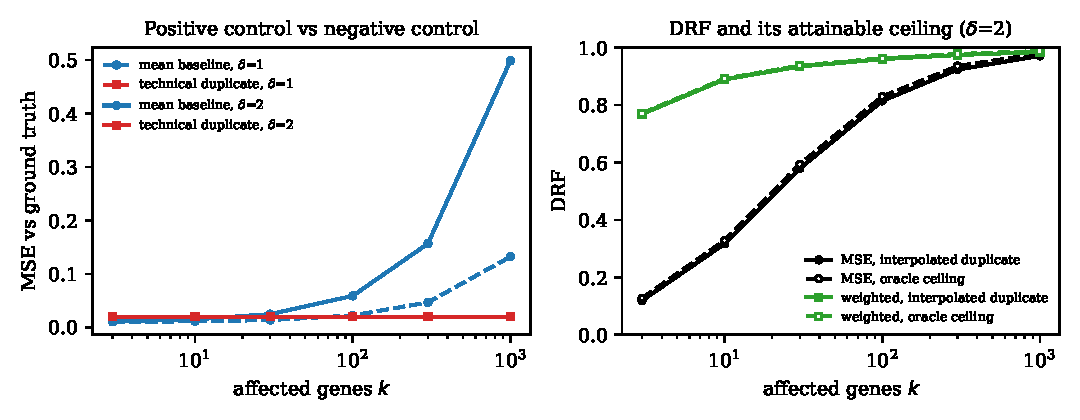
\includegraphics[width=\textwidth]{fig_calib.pdf}
\caption{Toy model. Left: error of the mean baseline and the technical duplicate against the number of affected genes $k$ for two shift sizes $\delta$; the curves cross where $k\delta^2=G/n_{TD}$. Right: DRF of the interpolated duplicate (solid) and of an oracle that knows the true profile (dashed), for squared error (black) and a significance-weighted squared error (green), $\delta=2$.}
\end{figure}

\section{The denominator is not attainable}

The ideal response in the denominator of DRF is the distance from the negative control to a perfect score. A perfect score against a ground truth that is itself the mean of $n_{GT}$ cells is not available to any predictor that has not seen those cells. The best a predictor can do is output the true profile $\mu$, which has expected error $1/n_{GT}$ against the ground truth, not zero. In the model, the DRF of this oracle is
\[
\DRF_{\mathrm{oracle}}(\mathrm{MSE})=\frac{k\delta^2/G}{k\delta^2/G+1/n_{GT}} ,
\]
which is the ceiling for any prediction under squared error. For $k=3$, $\delta=2$, $G=8192$ and $n_{GT}=100$ this is $0.13$. A predictor with exact knowledge of the true effects would therefore register a DRF of about $0.13$ under squared error, and a measured value of that size would not indicate that the metric fails to register model quality. It would indicate that the ground truth is too noisy for any prediction to do better.

\begin{table}[t]
\centering
\caption{DRF of the interpolated duplicate and of an oracle with the true profile, $\delta=2$, same simulation as Table~1. The weighted metric uses weights $1-P_{\mathrm{adj}}$ from the ground-truth half, in the spirit of, but not identical to, the weighted squared error of \citet{miller2026}.}
\begin{tabular}{rcccc}
\toprule
 & \multicolumn{2}{c}{Squared error} & \multicolumn{2}{c}{Weighted squared error} \\
$k$ & interpolated & oracle ceiling & interpolated & oracle ceiling \\
\midrule
3   & 0.120 & 0.128 & 0.769 & 0.772 \\
10  & 0.317 & 0.329 & 0.890 & 0.892 \\
30  & 0.579 & 0.594 & 0.935 & 0.937 \\
100 & 0.815 & 0.830 & 0.960 & 0.964 \\
\bottomrule
\end{tabular}
\end{table}

Table~2 shows two features. The interpolated duplicate comes within about 0.015 of the ceiling in every row, so in the model it is close to the best achievable positive control. And the ceiling for squared error is itself low in the sparse regime, so the raw DRF mixes two quantities: how sensitive the metric is to model quality, and how noisy the ground truth is. Datasets with fewer cells per perturbation have lower ceilings under any metric, and comparisons of DRF across datasets with different cell counts compare both. The paper's Supplementary Note~2 reports a downsampling analysis on Norman19 in which DRF rises monotonically with the number of cells for every metric examined. Under squared error it is approximately zero at 8 cells and $0.17$ at 64 cells, and under weighted squared error it is $0.61$ at 64 cells \citep{miller2026supp}. The Methods state that, at each target count $n$, $n/2$ cells are sampled from each half, so the ground-truth half and the positive-control half are degraded together \citep{miller2026}. The sweep therefore shows that calibration depends on sampling depth, as the authors say, but it cannot separate the loss of positive-control quality from the rise in the ground-truth noise floor, which both move with $n$. The point here is conceptual. A calibration report that gives DRF without the attainable ceiling invites a reading in which every shortfall is attributed to the metric.

The weighted metric in Table~2 has a ceiling near one even at $k=3$. This is expected, since it places most of its weight on the affected genes and so removes most of the noise floor. Section~5 considers what it loses in exchange.

\section{Sensitivity bought by weighting}

A metric that gains sensitivity by concentrating weight on the genes that the ground truth shows to be affected also stops penalizing errors elsewhere. A predictor that is correct on the affected genes and noisy on the rest then scores well. The paper recognizes this. It states that direct error metrics ``are a useful guardrail against rewarding implausible model predictions,'' and that ``a model performing substantially below baselines on either metric would warrant scrutiny regardless of calibration,'' where the two metrics in question are mean squared and mean absolute error \citep{miller2026}. The following illustrates why that caution carries weight.

Define a failure control: a predictor equal to the true profile plus independent noise of standard deviation $0.3$ on every gene. It captures the signal exactly and adds spurious structure.

\begin{table}[t]
\centering
\caption{Score relative to the mean baseline (lower is better; $1.0$ means no better than the mean baseline). The failure control is the true profile plus noise of standard deviation $0.3$ on every gene. $\delta=2$, same simulation.}
\begin{tabular}{rcccc}
\toprule
 & \multicolumn{2}{c}{Squared error} & \multicolumn{2}{c}{Weighted squared error} \\
$k$ & failure control & oracle & failure control & oracle \\
\midrule
3   & 8.73 & 0.87 & 0.88 & 0.22 \\
10  & 6.72 & 0.67 & 0.40 & 0.11 \\
30  & 4.05 & 0.41 & 0.22 & 0.06 \\
100 & 1.70 & 0.17 & 0.14 & 0.04 \\
\bottomrule
\end{tabular}
\end{table}

At $k=10$, squared error scores the failure control $6.7$ times worse than the mean baseline, and the weighted metric scores it $60\%$ better. The two metrics rank the same predictor on opposite sides of the negative control. Neither is wrong about what it measures. The weighted metric answers the question of whether the predictor captures the signal on the affected genes, and squared error answers the question of whether it avoids damaging the rest. A calibration protocol that checks only whether a metric separates a positive control from a negative one optimizes the first question. It has no way to detect the loss of the second, because no control in it is designed to fail in that way.

This suggests a third control class. A calibration should be reported against a positive control, a negative control, and at least one failure control that is right where the metric looks and wrong where it does not. A metric that rates all three sensibly has been shown to be sensitive without being blind in the way Table~3 displays. The concern was raised in review. A first-round reviewer noted that a challenge on virtual cell prediction had allowed submissions with exaggerated fold changes, and in places negative expression, to climb a leaderboard because neither differential-expression nor retrieval metrics alone captures overall realism, and asked that absolute-error metrics complement the calibrated ones \citep{miller2026peer}. The published text carries the guardrail language quoted above.

\section{Resolution, calibration and range}

Three properties of a benchmark comparison are often discussed as one.

\paragraph{Resolution} is whether the difference between two predictors on a given metric can be distinguished from sampling variation. It improves with more perturbations and with pairing, since a paired comparison across perturbations removes variation between perturbations. In Figure~2 of the paper, paired tests of models and baselines against the mean baseline over 2045 perturbations (Replogle22 K562) and 187 (Wessels23) give $t$ statistics in magnitude from about $1$ to above $45$, with Bonferroni-adjusted $P$ values as small as $10^{-309}$ \citep{miller2026}.

\paragraph{Calibration} is whether the metric's scale registers the property of interest, measured against controls. DRF is computed per perturbation and does not depend on the number of perturbations, whereas a $t$ statistic grows as the square root of that number. With enough perturbations a difference that is a few percent of the range is significant at any threshold. Significance and calibration therefore answer different questions, and a very small $P$ value under a poorly calibrated metric says that a small effect is reliably nonzero, not that the effect is large relative to what is possible.

\paragraph{Range} is how much room the benchmark leaves between the floor and the ceiling. Dilution compresses the room from below, as Section~3 showed. Saturation compresses it from above. The paper reports the second case for Norman19, where the additive baseline, which predicts a double perturbation as the sum of the two single ones, captures about $88\%$ of the ideal performance gap under the best-calibrated metrics, comparable to the interpolated duplicate that has access to held-out combination data, and where the training split covers $0.63\%$ of possible combinations. The authors infer a limit on the dataset's value for judging models that learn nonadditive interactions and recommend against using it alone \citep{miller2026}. In the Wessels23 dataset the training split covers $10.3\%$ of possible combinations, and the paper reports that PRESAGE exceeds the additive baseline on 15 of 18 metrics. A benchmark whose best baseline already realizes most of the range cannot rank models above that baseline, for the same structural reason that a diluted metric cannot rank models above the mean baseline.

The three properties combine. A comparison can have high resolution, low calibration and little range at once, and its $P$ value conveys none of the last two.

\section{What the conclusion licenses}

The paper's title is that deep-learning models ``can outperform baselines on calibrated metrics.'' This is an existence claim relative to a defined set of metrics, and it is what the evidence in the paper supports. It follows that the earlier reports of no advantage are uninformative about existence when the metrics used have low DRF, because a null result from an insensitive instrument is not evidence of absence. The paper makes this argument and supports it with the technical-duplicate analysis and the per-perturbation examples, such as a transcription factor perturbation with a DRF near zero for squared error whose differential-expression profile nonetheless recovers the factor's known binding targets in an enrichment analysis \citep{miller2026}.

Several things the conclusion does not establish are worth stating.

First, calibration is defined relative to the positive control. The interpolated duplicate is constructed from differential-expression significance on one half of the cells, and the weighted metrics are constructed from differential-expression significance on the other half. The halves are independent, so there is no leakage. But both encode the same notion of which genes carry the signal, so a high DRF for a weighted metric partly measures agreement between the metric and the control about what the signal is. The paper addresses this in Supplementary Note~2 by recomputing DRF with the control-cell baseline as the negative control and the technical duplicate as the positive control. Absolute DRF values change, but the metrics ranked highest by calibration remain largely the same, and mean absolute error is poorly calibrated in every case. The technical duplicate as positive control gave negative calibration in several weaker-perturbation datasets for the metrics least sensitive to perturbation-specific signal, which is the failure of Section~3, while the retrieval metrics (PDS and NIR) stayed well calibrated, since they do not depend on the size of the error \citep{miller2026supp}. The alternatives examined are close relatives of the original controls, since all are built from the same cells and the same reference mean. A first-round reviewer asked how the ranking of metrics would change under a structurally different trivial baseline, one that is informative on retrieval and poor on delta metrics, and the supplement does not report such a baseline \citep{miller2026peer}. Whether the identification is stable under controls that define signal in a more different way remains open.

Second, the metrics disagree about models. The paper reports that scGPT attains the lowest weighted squared error among the models on one dataset ($0.027\pm0.001$) and the highest correlation on differentially expressed genes ($0.367\pm0.009$), yet scores $0.081\pm0.003$ on the correlation of perturbation-referenced deltas over all genes, which the authors describe as barely above the mean baseline. The authors caution against treating any single well-calibrated metric as definitive \citep{miller2026}. The failure-control analysis of Section~5 gives a mechanism by which such disagreements arise: metrics that look at different genes can rate the same predictor differently. The supplement adds a related observation. Across perturbations of increasing strength, positive-control performance under the retrieval and fit-based calibrated metrics (NIR and weighted $R^2$) improves, but under weighted squared error, as under squared error, the trend is weak or non-monotonic, which the authors attribute to larger shifts being harder to reconstruct point by point \citep{miller2026supp}. A reviewer remarked that a unified statement that well-calibrated metrics respond to perturbation strength is therefore an overstatement for that metric \citep{miller2026peer}.

Third, the downstream agreement reported between model rankings under calibrated metrics and rankings by pathway recovery ($\rho=0.76$ and $0.84$ in two datasets) and by neighborhood-structure recovery ($0.77$ and $0.58$) is a correlation computed over a small number of models and baselines, and its sampling variability is large for that number. It supports consistency, not a precise measurement of how closely calibrated metrics track biological recovery.

None of these undermines the paper's claim. They mark the distance between ``the metrics used in earlier null results were insensitive'' and ``the models predict perturbation biology well enough to use,'' which the paper does not assert.

\section{Reporting practices}

The analysis suggests six practices for benchmarks of this kind. Each is stated as a requirement on what a reader should be able to find.

\begin{enumerate}
\item The scores of the negative and positive controls should appear in the same table as the model, so that a model score can be read against both.
\item An attainable ceiling should accompany any ratio against ``perfect'' performance, computed from the noise of the ground truth, as in Section~4. A shortfall relative to perfection is not a shortfall relative to what is achievable.
\item At least one failure control should be reported, a predictor that is correct where the metric looks and wrong elsewhere, so that sensitivity is not purchased with blindness.
\item Effects should be reported as fractions of the available range with intervals across units, in addition to any significance test, because significance depends on the number of units and range fractions do not.
\item When the best baseline realizes most of the range, the benchmark should be described as unable to rank models above it, as the paper does for Norman19.
\item Agreement between metric families should be reported with its uncertainty and with the number of models on which it rests.
\end{enumerate}

\section{Limits}

The model treats genes as independent, assumes homogeneous noise, assumes that the mean baseline equals the unperturbed profile, and uses a significance weighting that resembles but is not the weighted squared error of the paper. The values in the tables are properties of the toy model, chosen for $G$ near the 8192 genes the paper selects, and do not reproduce any dataset. The essay draws on the main text, Methods, Supplementary Notes~1 and 2, the supplementary tables and the peer review file of the paper, and on the legends but not the panels of the extended data figures. Statements about the prior benchmarks that the paper responds to are taken from the paper's description of them. The analysis addresses the logic of calibration and does not evaluate the empirical performance of any model.

\appendix
\section{Derivations}

\paragraph{Expected errors.} Write $y=\mu+e_{GT}$ and $\hat y_{TD}=\mu+e_{TD}$ with independent $e_{GT,g}\sim N(0,1/n_{GT})$ and $e_{TD,g}\sim N(0,1/n_{TD})$. For the negative control $\hat y_n=0$, $\E(y_g-0)^2=\mu_g^2+1/n_{GT}$, and summing over $g$ and dividing by $G$ gives $k\delta^2/G+1/n_{GT}$. For the duplicate, $\E(y_g-\hat y_{TD,g})^2=1/n_{GT}+1/n_{TD}$ for every gene. The inequality follows by subtraction.

\paragraph{Shrinkage weight.} For one gene, the error of $\alpha\hat y_{TD}+(1-\alpha)\cdot0$ against $\mu_g$ has expectation $\alpha^2/n_{TD}+(1-\alpha)^2\mu_g^2$. Setting the derivative to zero gives $\alpha=\mu_g^2/(\mu_g^2+1/n_{TD})$.

\paragraph{Oracle ceiling.} The prediction $\mu$ has $\E\,\mathrm{MSE}=1/n_{GT}$ against $y$. Then $\DRF=(\mathrm{MSE}_n-\mathrm{MSE}_{or})/\mathrm{MSE}_n=(k\delta^2/G)/(k\delta^2/G+1/n_{GT})$.

\paragraph{Invariance.} If $m'=am+b$ then $m'(\hat y_p)-m'(\hat y_n)=a[m(\hat y_p)-m(\hat y_n)]$ and $m'(y)-m'(\hat y_n)=a[m(y)-m(\hat y_n)]$, so the ratio is unchanged when $\epsilon=0$.

\section{Simulation details}

Each simulated perturbation draws $k$ affected genes uniformly from $G=8192$, assigns each a shift of $+\delta$ or $-\delta$ with equal probability, and draws the ground-truth half and technical-duplicate half as independent noisy means with $n_{GT}=n_{TD}=100$. The technical-duplicate $z$ scores are converted to two-sided normal $P$ values, adjusted across genes with the Benjamini--Hochberg procedure, and the interpolation weight is one minus the adjusted $P$ value. The weighted metric uses weights equal to one minus the adjusted $P$ value from the ground-truth half, normalized to mean one. Each table row averages 300 simulated perturbations with a fixed seed. The failure control adds independent Gaussian noise of standard deviation $0.3$ to the true profile. The script \texttt{calib.py} reproduces every number and the figure.

\begin{thebibliography}{9}
\bibitem[Miller et al.(2026a)]{miller2026}
H.~E. Miller, G.~M. Mejia, F.~J.~A. Leblanc, B.~Swain, B.~Wang and L.~P. de Lima Camillo.
\newblock Deep learning perturbation models can outperform baselines on calibrated metrics.
\newblock \emph{Nature Biotechnology}, 2026. doi:10.1038/s41587-026-03307-w.

\bibitem[Miller et al.(2026b)]{miller2026supp}
H.~E. Miller et al.
\newblock Supplementary information for \emph{Deep learning perturbation models can outperform baselines on calibrated metrics}, Supplementary Notes 1 and 2.
\newblock \emph{Nature Biotechnology}, 2026.

\bibitem[Miller et al.(2026c)]{miller2026peer}
\newblock Peer review file for \emph{Deep learning perturbation models can outperform baselines on calibrated metrics}.
\newblock \emph{Nature Biotechnology}, 2026.

\bibitem[Benjamini and Hochberg(1995)]{bh1995}
Y.~Benjamini and Y.~Hochberg.
\newblock Controlling the false discovery rate: a practical and powerful approach to multiple testing.
\newblock \emph{Journal of the Royal Statistical Society, Series B}, 57(1):289--300, 1995.
\end{thebibliography}

\end{document}
